	\documentclass{report}
	\usepackage[T1]{fontenc}
	\usepackage[utf8]{inputenc}
	\usepackage[english]{babel}
	
	\usepackage[dvipsnames]{xcolor}
	
	\usepackage{tikz,pgfplots,pgfplotstable,pgffor,pgfmath,tikz-3dplot}
	\pgfplotsset{compat=newest}
	
	%===================================================
	\usetikzlibrary{positioning,plotmarks,pgfplots.colormaps,external,3d,calc,arrows}
	\usetikzlibrary{decorations,decorations.pathmorphing,decorations.pathreplacing}
	\usetikzlibrary{shapes,arrows}
	\tikzexternalize[mode=convert with system call,shell escape=-enable-write18]
	%===================================================
	
	
	
	%==== Tikz & PGF Camera alignment macro ============
	% Style to set TikZ camera angle, like PGFPlots `view`
	\tikzset{viewport/.style 2 args={
	    x={({cos(-#1)*1cm},{sin(-#1)*sin(#2)*1cm})},
	    y={({-sin(-#1)*1cm},{cos(-#1)*sin(#2)*1cm})},
	    z={(0,{cos(#2)*1cm})}
	}}
	%===================================================
	
	%==== Z Buffer Stuff ======================================
	% Styles to plot only points that are before or behind the sphere.
	\pgfplotsset{only foreground/.style={
		restrict expr to domain={rawx*\CameraX + rawy*\CameraY + rawz*\CameraZ}{-0.05:100},
	}}
	\pgfplotsset{only background/.style={
		restrict expr to domain={rawx*\CameraX + rawy*\CameraY + rawz*\CameraZ}{-100:0.05}
	}}
	
	% Automatically plot transparent lines in background and solid lines in foreground
	\def\addFGBGplot[#1]#2;{
		\addplot3[#1,only background, opacity=0.25] #2;
		\addplot3[#1,only foreground] #2;
	}
	%===================================================
	
	
	% Define standard arrow tip ========================
	\tikzset{>=stealth',}
	%===================================================
	
	% Custom Color Map =================================
	\pgfplotsset{ % Note: use colors in Capital letters, they are the proper ones from xcolor package
		colormap={colormapGray}{
			color(0cm)=(White!10!Black);
			color(1cm)=(White)
		},
		colormap={colormapBlue}{
			color(0cm)=(White!20!Black);
			color(1cm)=(Blue)
		}
	}
	%===================================================
	
	\begin{document}
	
	%== use predefined colormaps
	%\newcommand{\colormap}{colormap/gray}%/redyellow}%/winter}%/cool}
	%== use custom colormaps
	\newcommand{\colormap}{colormap name={colormapGray}}
	
	
	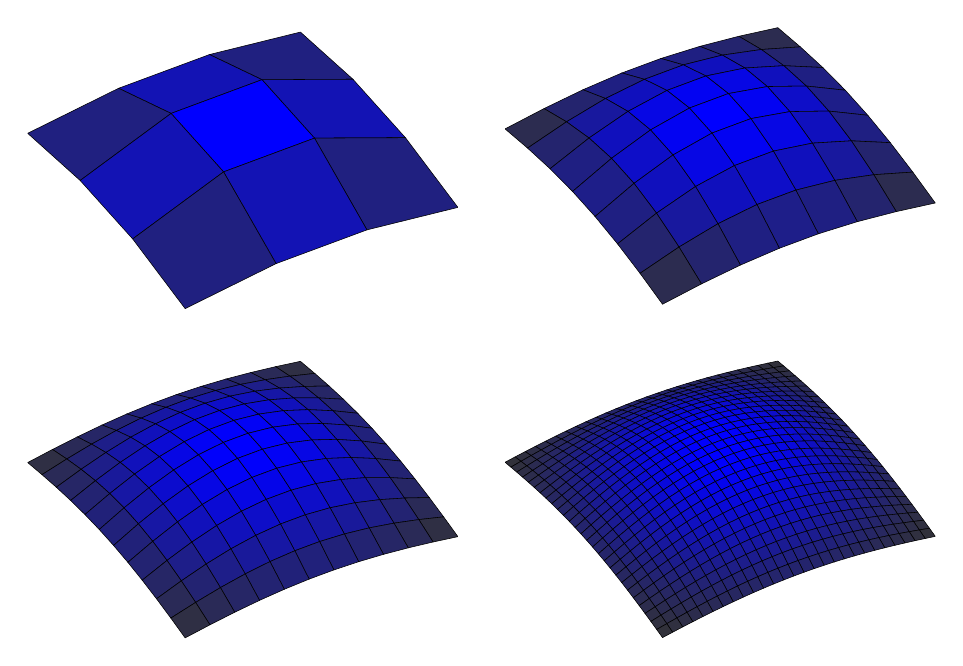
\begin{tikzpicture}
	
		\newcommand{\radius}{5}
		\newcommand{\ViewAzimuth}{-210}
		\newcommand{\ViewElevation}{40}
		
		% Compute camera unit vector for calculating depth
		\pgfmathsetmacro{\CameraX}{sin(\ViewAzimuth)*cos(\ViewElevation)}
		\pgfmathsetmacro{\CameraY}{-cos(\ViewAzimuth)*cos(\ViewElevation)}
		\pgfmathsetmacro{\CameraZ}{sin(\ViewElevation)}
		%\path[use as bounding box] (-{(\radius*0.4)},-{(\radius*0.5)}) rectangle ({(\radius)},{(\radius*0.8)}); % Avoid jittering animation
		
		%%%% Top left
		\begin{axis}
		[
			scale only axis,
			hide axis,
			view={\ViewAzimuth}{\ViewElevation},     % Set view angle
			every axis plot/.style={very thin},
			disabledatascaling,                      % Align PGFPlots coordinates with TikZ
			anchor=origin,                           % Align PGFPlots coordinates with TikZ
			viewport={\ViewAzimuth}{\ViewElevation}, % Align PGFPlots coordinates with TikZ
			\colormap
		]
			
			% Sphere =====================
			\addplot3[
			% surf          - surface plot
			% shader=flat   - no interpolation, one face has one color remove for fluent transitions
			% draw=black    - customise this to change the grid lines, e.g. draw={red!50!black,thick,...}
			% z buffer=sort - weiß ich selber nicht genau
			% \colormap     - der befehl ist oben definiert, hier auskommentiert da über die axis verwendet (custom color map). bei predefined color maps kann man die bei jedem plot einzeln festlegen
			% point meta=z  - was codiert die colormap (zB ..=-z um die map zu invertieren)
			% samples=n     - die anzahl der samples (x und y; kann auch für x und y separat gesetzt werden)
			% domain=x_min:x_max - x domain für das sampling
			% y domain=...  - selbsterklärend
				surf, shader=flat, draw=black, z buffer=sort, point meta=z,
				samples=4, domain=-0.4*pi:0.4*pi, y domain=-0.4*pi:0.4*pi%, \colormap
			]
			(
				\radius * x / pi, % X coordinate
				\radius * y / pi, % Y coordinate
				{cos(deg(x)) * cos(deg(y))}  % Z (vertical) coordinate
			);
			
%		
%			% Coordinate System
%			\draw[->,very thick] (0,0,0) -- (0,0,\radius) node[anchor=north east,below left=-0.3 and -0.15]{$z$};
%			\draw[->,very thick] (0,0,0) -- (0,\radius,0) node[anchor=north east]{$y$};
%			\draw[->,very thick] (0,0,0) -- (\radius,0,0) node[anchor=north east]{$x$};
%			
%			
%			
%			% Plot equator and two longitude lines with occlusion
%			\addFGBGplot[red!70!black,domain=0:2*pi, samples=100, samples y=1,very thick] ({\radius*cos(deg(x))}, {\radius*sin(deg(x))}, 0);
%			\addFGBGplot[red!70!black,domain=0:2*pi, samples=100, samples y=1,very thick] (0, {\radius*sin(deg(x))}, {\radius*cos(deg(x))});
%			\addFGBGplot[red!70!black,domain=0:2*pi, samples=100, samples y=1,very thick] ({\radius*sin(deg(x))}, 0, {\radius*cos(deg(x))});
		
		
		\end{axis}
		
		
		%%%% Top right
		\begin{axis}
		[
			scale only axis,
			hide axis,
			view={\ViewAzimuth}{\ViewElevation},     % Set view angle
			every axis plot/.style={very thin},
			disabledatascaling,                      % Align PGFPlots coordinates with TikZ
			anchor=origin,                           % Align PGFPlots coordinates with TikZ
			viewport={\ViewAzimuth}{\ViewElevation}, % Align PGFPlots coordinates with TikZ
			at={(0.5\linewidth,0)},	 				 % Position
			\colormap
		]
			\addplot3[
				surf, shader=flat, draw=black, z buffer=sort, point meta=z,
				samples=8, domain=-0.4*pi:0.4*pi, y domain=-0.4*pi:0.4*pi%, \colormap
			]
			(
				\radius * x / pi, % X coordinate
				\radius * y / pi, % Y coordinate
				{cos(deg(x)) * cos(deg(y))}  % Z (vertical) coordinate
			);
			%=============================
		\end{axis}
		
		%%%%% Bottom left
		\begin{axis}
		[
			scale only axis,
			hide axis,
			view={\ViewAzimuth}{\ViewElevation},     % Set view angle
			every axis plot/.style={very thin},
			disabledatascaling,                      % Align PGFPlots coordinates with TikZ
			anchor=origin,                           % Align PGFPlots coordinates with TikZ
			viewport={\ViewAzimuth}{\ViewElevation}, % Align PGFPlots coordinates with TikZ
			at={(0,-0.35\linewidth)},	 			 % Position
			\colormap
		]
		
			% Sphere
			\addplot3[
				surf, shader=flat, draw=black, z buffer=sort, point meta=z,
				samples=12, domain=-0.4*pi:0.4*pi, y domain=-0.4*pi:0.4*pi%, \colormap
			]
			(
				\radius * x / pi, % X coordinate
				\radius * y / pi, % Y coordinate
				{cos(deg(x)) * cos(deg(y))}  % Z (vertical) coordinate
			);
		
		\end{axis}
		
		%%%%% Bottom right
		\begin{axis}
		[
			scale only axis,
			hide axis,
			view={\ViewAzimuth}{\ViewElevation},     % Set view angle
			every axis plot/.style={very thin},
			disabledatascaling,                      % Align PGFPlots coordinates with TikZ
			anchor=origin,                           % Align PGFPlots coordinates with TikZ
			viewport={\ViewAzimuth}{\ViewElevation}, % Align PGFPlots coordinates with TikZ
			at={(0.5\linewidth,-0.35\linewidth)},	 % Position
			\colormap
		]
		
			% Sphere
			\addplot3[
				surf, shader=flat, draw=black, z buffer=sort, point meta=z,
				samples=28, domain=-0.4*pi:0.4*pi, y domain=-0.4*pi:0.4*pi%, \colormap
			]
			(
				\radius * x / pi, % X coordinate
				\radius * y / pi, % Y coordinate
				{cos(deg(x)) * cos(deg(y))}  % Z (vertical) coordinate
			);
		
		\end{axis}
		
	\end{tikzpicture}
	
	\end{document}